\documentclass[a4paper,10pt]{article}

\usepackage{adjustbox}
\usepackage{graphicx}
\usepackage{hyperref}
\usepackage{minted}
\usepackage{amsmath}
%opening
\title{The Memory \& Storage Design of Neo4J}
\author{Fabian Klopfer}

\begin{document}

\maketitle
\vspace{2cm}

\begin{abstract}
In this document I describe the internals of the storage layer of the popular native graph database Neo4J. A detailed description of how records are stored into which files and how these are accessed is to be elaborated on in the following article. This is a translation, update and extension of previous work done by Michael Brendle. Further the page cache (or buffer manager) and examples on access patterns generated by graph traversals are given. This is done in order to gain insights and prepare for optimizing locality on the storage level to minimize IO.
\end{abstract} \newpage

\tableofcontents \newpage

\section{Introduction}
Relational databases store tables of data. The links considered in this category of DBMS are mostly used to stitch together the fields of an entry into one row again, after it has been split to satisfy a certain normal form. Of course one may also store tables where one table stores nodes and the other table's fields are node IDs to represent relationships.

However, in order to traverse the graph, one has either to do a lot of rather expensive look ups or store auxiliary structures to speed up the look up process. In particular when using B-trees as index structure, each look up takes $\mathcal{O}(\log(n))$ steps to locate a specific edge. Alternatively one could store an additional table that holds edge lists such that the look up of outgoing or incomming edges is only $\mathcal{O}(\log(n))$ which would speed up breadth first traversals. But still one has to compute joins in order to continue the traversal in terms of depth. Another way to speed things up is to use a hash-based index, but this also has a certain overhead aside from the joins.

In contrast to relational data base management systems, native graph data\-bases use structures specialised for this kind of queries. In the remainder of the document I discuss based upon Michael Brendle's work what structures and mechanisms the graph database Neo4J uses in order to achieve this superior performance in the domain of graphs.

First of all, let us consider the high level architecture of a database management systems as shown in figure~\ref{dbms_arch} --- with a focus on the storage and loading elements.

\begin{figure}[htp]\label{dbms_arch}
 \begin{center}
  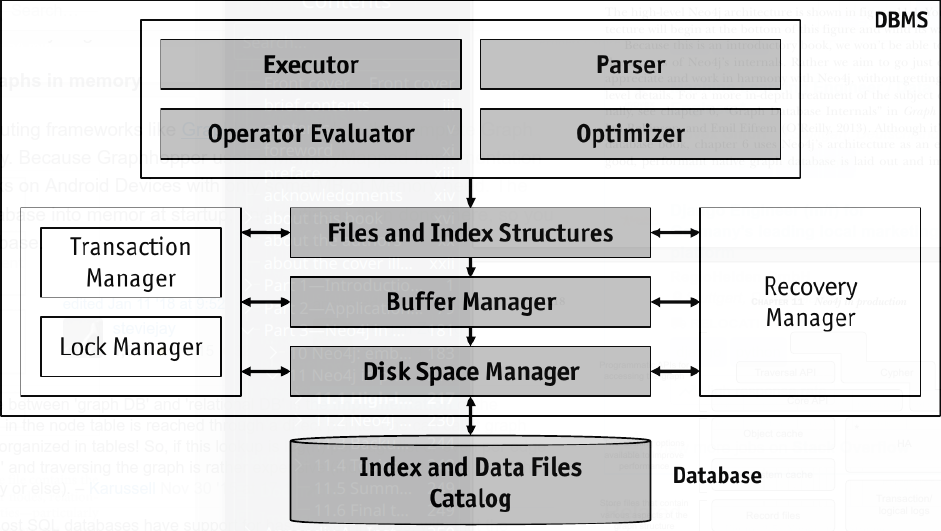
\includegraphics[keepaspectratio,width=0.7\textwidth]{img/intro/RDBMS.png}
 \end{center}
 \caption{The typical structure of a relational database management system.} %TODO citation
\end{figure}

Here The disk space manager, sometimes also called storage manager, handles de-/allocations, reads \& writes and provides the concept of a page: A disk block brought into memory. For that it needs to keep track of free blocks in the allocated file. Optimally both a disk block and a page are of the same size. One crucial task of a disk space manager is to store sequences of pages into continuous memory blocks in order to optimize data locality. Data locality has the upside, that one needs only one I/O operation to load multiple pages. To summarize the two most important objectives of a storage manager are to provide a locality-preserving mapping from pages to blocks based upon the information in the DBMS and to abstract physical storage to pages, taking care of allocation and access.
A buffer manager is used to mediate between external storage and main memory. It maintains a designated pre-allocated area of main memory --- called the buffer pool --- to load, cache and evict pages into or from main memory. It's objective is to minimize the number of disk reads to be executed by caching, pre-fetching and the usage of suitable replacement policies. It also needs to take care of allocating a certain fraction of pages to each transaction.

\begin{figure}[htp]\label{dbms_memory}
    \begin{center}
    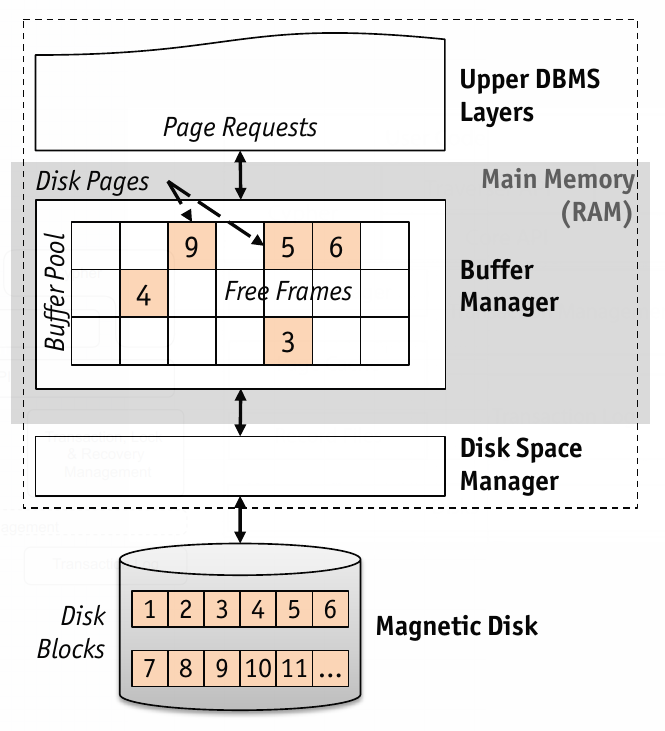
\includegraphics[keepaspectratio,height=0.4\textheight,width=0.5\textwidth]{img/intro/RDBMS_memory_view.png}
    \end{center}
    \caption{A visualization of the interaction of a database with memory.} %TODO citation
\end{figure}

The final memory and storage model relevant component of the  of a database management system is the file layout and possible index structures. 
In order to store data a DBMS may either store one single or multiple files to maintain records. 

A file may consist of a set of pages containing a set of slots. A slot stores one record with each record containing a set of fields. Further the database needs to keep track of free space in the file: A linked list or a directory must record free pages and some structure needs to keep track of the free slots either globally or per page. 

Records may be of fixed or of variable size, depending on the types of their fields. Records can be layout in row or column major order. That is one can store sequences of tuples or sequences of fields. The former is beneficial if a lot of update, insert or delete operations are committed to the database, while the latter optimizes the performance when scans and aggregations are the most typical queries to the system.

Another option is to store the structure of the records along with pointers to the values of their fields in one files and the actual values in one or multiple separate files. Also distinct types of tables can be stored in different files. For example entities and relations can be stored in different files with references to each other, thus enabling the layout of these two to be specialized to their structure and usage in queries.

Files may either organize their records in random order (heap file), sorted or using a hash function on one or more fields. All of these approaches have upsides and downsides when it comes to scans, searches, insertions, deletions and updates. 

To mitigate the effect that result from selecting one file organization or another, the concept of indexes have been introduced. Indexes are auxiliary structures to speed up certain operations that depend on one field. Indexes may be clustered or unclustered. An index over field $F$ is called clustered if the underlying data file is sorted according to the values of $F$. An unclustered index over field $G$ is one where the file is not sorted according to $G$. In a similar way indexes can be sparse or dense. A sparse index has less index entries than records, mostly one index entry per file. This can of course only be done for clustered indexes as the sorting of the data file keeps the elements between index keys in order. An index is dense if there is a one to one correspondence between records and index entries. There are different variants of storing index entries which have again certain implications on the compactness of the index and the underlying design decisions.

In another view of database management systems architectures, this boils down to the design decisions one has to make when implementing the storage layer and the access layer as shown in figure~\ref{dbms_arch_layers}.

\begin{figure}[htp]\label{dbms_arch_layers}
 \begin{center}
  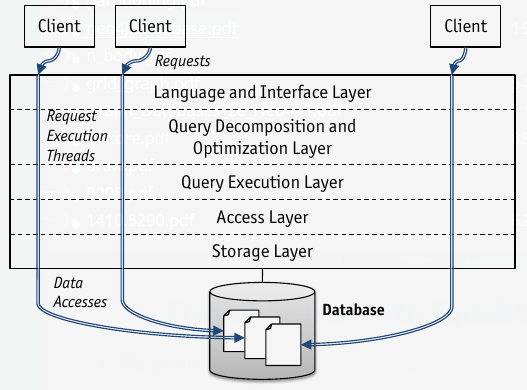
\includegraphics[keepaspectratio,width=0.6\textwidth]{img/intro/layered_RDBMS.png}
 \end{center}
 \caption{The architecture of a database management system from another point of view.} %TODO citation
\end{figure}

Here the storage layer is in close correspondence to the disk space manager in combination with the buffer manager, while the files and index structures provide the access layer.

All these considerations make choosing different file splits, layouts, orderings, addressing schemes, management structures, de-/allocation schemes and indexes a complex set of dependent choices. 
These depend mainly on the structure of the data to be stored and the queries to be run. 

When restricting to graph structures where nodes and relationships are allowed to have properties and labels and types respectively, this allows one to narrow down some of the design decisions. In particular the example of a popular graph native database --- Neo4J --- is what I discuss in the next sections. 

To get an overview of the architecture let us consider figure~\ref{N4J_HLA_Emil}. 

\begin{figure}[htp]\label{N4J_HLA_Emil}
 \begin{center}
  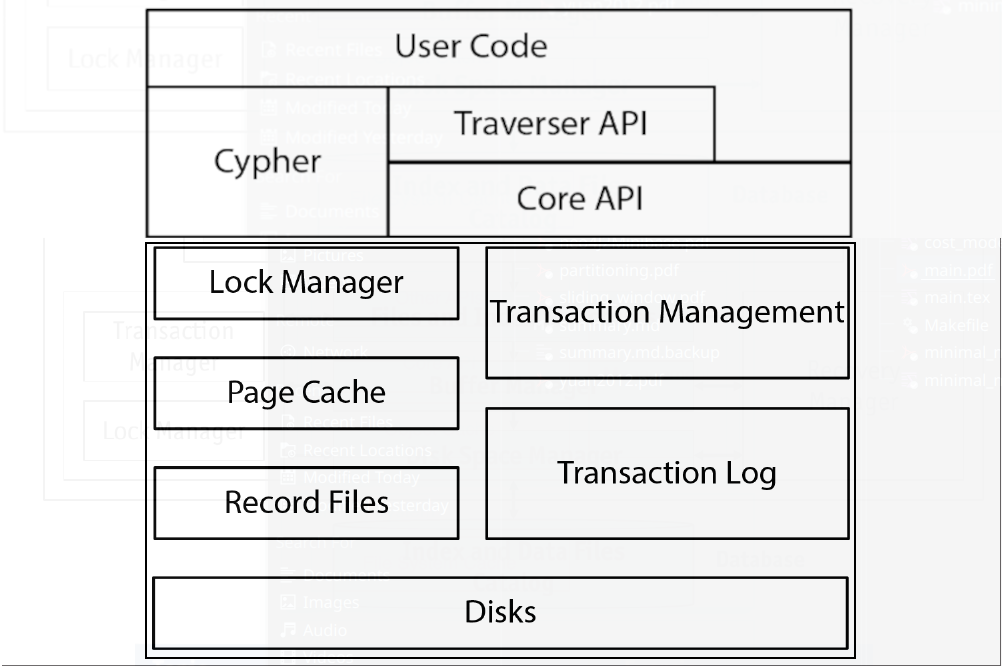
\includegraphics[keepaspectratio,width=0.6\textwidth]{img/intro/N4J_HLA_Emil.png}
 \end{center}
 \caption{The high level architecture of Neo4J according to Emil Efrim, the co-founder of Neo technologies.} %TODO citation
\end{figure}

Here we can see that the previous schema is not exactly straight forward to apply, mainly due to a lack of concise documentation. The diagram was taken from the only publication that elaborates on the internals of Neo4J aside from the code of course. Here The storage manager makes mostly use of the Java NIO package with some additional usage of operating system native calls to allocate memory for the page cache and network buffers. 
A more detailed view on the high level architecture of the disk space and buffer manager and the fiels and index structures was deduced by the author from the source code and the non-public JavaDocs. This is shown in figure~\ref{N4J_Storage}.

\begin{figure}[htp]\label{N4J_Storage}
 \begin{center}
  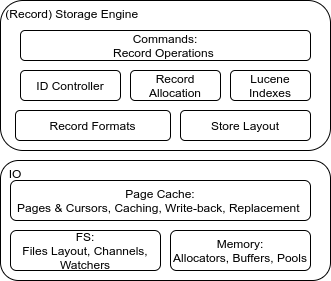
\includegraphics[keepaspectratio,width=0.5\textwidth]{img/intro/N4J_Storage.png}
 \end{center}
 \caption{A visualization of the broad the storage and memory organization of Neo4J.} %TODO citation
\end{figure}

In the next section the focus is set on the storage layer of Neo4J: How it handles allocations, read and writes and how it provides the notion of a page. After that I elaborate on the details of the page cache, the transformation it applies to nodes and relationships on loading, the caching and the page eviction strategies it employs. Finally the internals of the files and records layouts are discussed along with the special structures employed and the indexes that are (or may be ) created over the files.

The overall memory and storage state of a Neo4J instance and its environment may thus be visualized like this figure~\ref{N4J_memory_view}.

\begin{figure}[htp]\label{N4J_memory_view}
 \begin{center}
  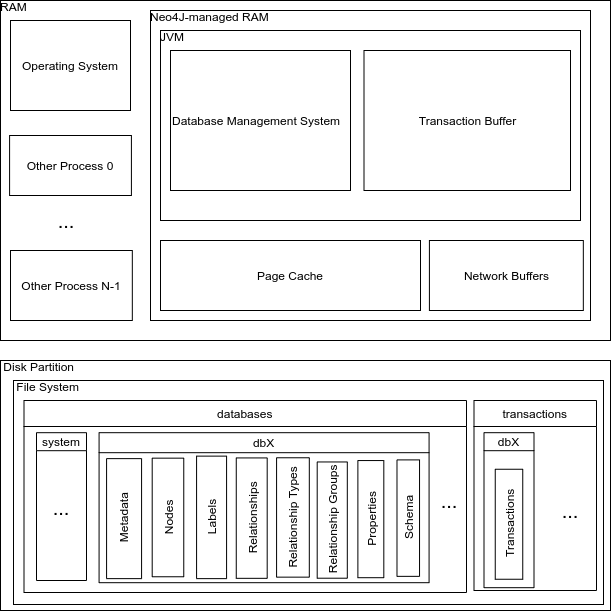
\includegraphics[keepaspectratio,width=\textwidth]{img/intro/N4J_memory_view.png}
 \end{center}
 \caption{A sketch of how Neo4J occupies memory.} %TODO citation
\end{figure}


\section{Disk Space Management}
TODO later
\mintinline{bash}{neo4j/community/io/src/main/java/org/neo4j/io/(fs|mem|memory)} \\
\mintinline{bash}{neo4j/community/native} \\
\href{http://g-store.sourceforge.net/th/index.htm}{G-Store} \\


\section{Buffer Management}
TODO later

\mintinline{bash}{
neo4j/community/io/src/main/java/org/neo4j/io/pagecache
} \\
\href{https://www.slideshare.net/thobe/an-overview-of-neo4j-internals}{Page Cache record layout} \\


\section{File, Record \& Index Structures}
\subsection{File Layout}
    
\subsection{Record Structures}
    \subsection{Address Translation}
    Neo4j defines the following constants as the size of the addresses used.
        \begin{figure}[H]\label{addrsize}
    \adjustbox{varwidth=\textwidth, scale=0.9}{%
    \begin{minted}[autogobble]{Java}
        public static final int PROPERTY_TOKEN_MAXIMUM_ID_BITS = 24;
        static final int NODE_MAXIMUM_ID_BITS = 35;
        static final int RELATIONSHIP_MAXIMUM_ID_BITS = 35;
        static final int PROPERTY_MAXIMUM_ID_BITS = 36;
        public static final int DYNAMIC_MAXIMUM_ID_BITS = 36;
        public static final int LABEL_TOKEN_MAXIMUM_ID_BITS = 32;
        public static final int RELATIONSHIP_TYPE_TOKEN_MAXIMUM_ID_BITS = 16;
        static final int RELATIONSHIP_GROUP_MAXIMUM_ID_BITS = 35;
        public static final int SCHEMA_RECORD_ID_BITS = 32;
     \end{minted}
     }
    \end{figure}
    These are represented by the datatype \mintinline{java}{long} when loaded into main memory. On disk these values are stored as 32-bit \mintinline{java}{Integer}s with additional modifiers, that is the highest bits that do not fit into an int are stored to fields with additional space.
    
    For example the in-use bit consumes one byte of memory and the additional 7 bytes are used to stroe the highest bits that do not fit into an integer of another field.
    
    Finally the base and the modifer are aggregated into a long by shifting both appropriately, casting them to longs and applying the logical or \mintinline{java}{|} operation.
    
    
    \subsubsection{Nodes}
    The record format of nodes consist of a 15 byte structure. The IDs of nodes are stored implicitly as their address. If a node has ID 100 we know that its record starts at offset $15 \text{ Bytes} \cdot 100 = 1500$ from the beginning of the file. The struct of a record looks like this:
    \begin{enumerate}
     \item Byte 1: The first byte contains one bit for the in-use flag. The additional 7 bits are used to store the 3 highest bits of the relationship ID and the 4 highest bits of a property ID
     \item Bytes 2 - 5: The next 4 Bytes represent the ID of the first relationship in the linked list containing the relationships of the considered node.
     \item Bytes 6 - 9: Again 4 bytes encode the ID to the first property of the node.
     \item Bytes 10 - 14: This 5 byte section points to the labels of this node, labels might also be inlined.
     \item Byte 15: The last byte stores if the node is dense, i.e. one node has an aweful lot of relationships and is treated a bit differently. That is a relationships are stored by type and direction for this node into groups, see~\ref{rel_group}.
    \end{enumerate}
    
    \begin{figure}[htp]\label{node_record}
    \begin{center}
    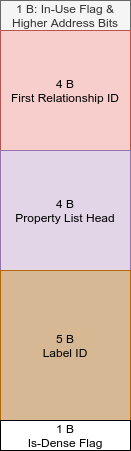
\includegraphics[keepaspectratio,height=0.4\textheight,width=0.5\textwidth]{img/node/node_record.png}
    \end{center}
    \caption{A visualization of the record structure of a node.} %TODO citation
    \end{figure}
     
    To summarize: The records on disk are stored as in the enumeration above. In the database all IDs get mapped to longs and their respective space is larger than the space representable by 35 bit --- what is perfectly fine.
    
    \begin{figure}[htp]\label{node_first_byte}
        \begin{center}
        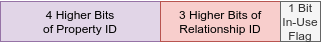
\includegraphics[keepaspectratio,height=0.4\textheight,width=0.5\textwidth]{img/node/node_first_byte.png}
        \end{center}
        \caption{A visualization of the information stored in the first byte of a node record.} %TODO citation
    \end{figure}
    
    On disk 4 byte integers are used to store the 32 lowest bits of the respective addresses and the higher bits are stored in the first byte that also carries the in-use bit.
    
    \subsubsection{Node Labels}
    Each node label record consists of an in use bit and a name ID, which in turn points to an entry in a seperate file storing label names as dynamic records (see \ref{dynamic}), storing the label names. This is done in order to asure that the records are of fixed length.
    \begin{enumerate}
     \item Byte 1: In-use flag
     \item Bytes 2-5: Pointer to the label string entry
    \end{enumerate}
    
    \begin{figure}[htp]\label{label_record}
        \begin{center}
            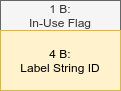
\includegraphics[keepaspectratio,height=0.2\textheight,width=0.2\textwidth]{img/node/label_record.png}
        \end{center}
        \caption{A visualization of the structure of a label record.} %TODO citation
    \end{figure}
    
    
    
    \subsubsection{Relationships}
    \begin{figure}[htp]\label{rel_record}
        \begin{center}
            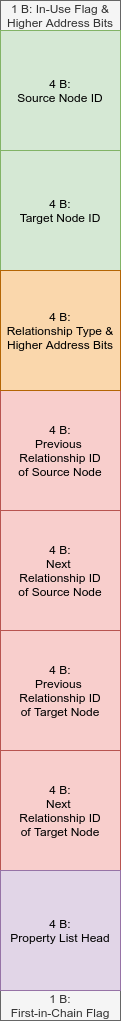
\includegraphics[keepaspectratio,height=0.9\textheight,width=0.5\textwidth]{img/relationship/relationship_record.png}
        \end{center}
        \caption{A visualization of the record structure of a relationship in Neo4J.} %TODO citation
    \end{figure}
    
    Relationship records are stored with implicit IDs too. Their fixed size records contain 34 bytes. Besides an in-use flag and the node IDs that are connected, and the relationship type, the record also contains two doubly linked list: One for the relationships of the first node and one for the relationship of the second node. Finally a link to the head of the properties linked list of this relationship and a marker if this relationship is the first element in the relationships linked list of one of the nodes.
    \newpage
    \begin{enumerate}
     \item Byte 1: In-use bit, first node high order bits (3 bits), first property high order bits (4 bits)
     \item Bytes 2 - 5: first node ID 
     \item Bytes 6 - 9: second node ID 
     \item Bytes 10 - 13: relationship type (16 bit), second node high order bits (3 bits), relationship previous and next ID higher bits for first and second node ($4 \cdot 3 = 12$ bits, one unused bit.
     \item Bytes 14 - 17: previous relationship ID for first node
     \item Bytes 18 - 21: next relationship ID for first node
     \item Bytes 22 - 25: previous relationship ID for second node
     \item Bytes 26 - 29: next relationship ID for second node
     \item Bytes 30 - 33: link to the first property of the relationship
     \item Bytes 34: A marker if this relation is the first element in the relationship linked list of one of the nodes stored in the lowest two bits of the byte. The other 6 bits are unused.
    \end{enumerate}


\begin{figure}[htp]\label{rel_first_byte}
 \begin{center}
  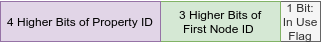
\includegraphics[keepaspectratio,width=\textwidth]{img/relationship/relationship_first_byte.png}
 \end{center}
 \caption{A visualization of how information is stored in the first byte of a relationship record.} %TODO citation
\end{figure}

\begin{figure}[htp]\label{rel_type_bytes}
 \begin{center}
  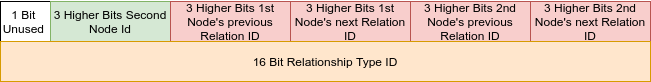
\includegraphics[keepaspectratio,width=\textwidth]{img/relationship/relationship_type_bytes.png}
 \end{center}
 \caption{The structure of the bytes that are used to store the type of a relationship and high bits of a node and a relationship IDs.} %TODO citation
\end{figure}
    

    \subsubsection{Relationship Types}
    Similarly to the node labels, the relationship type records posses an in-use flag and a type ID that points to a record in a file containing strings in the dynamic record format.
        \begin{enumerate}
     \item Byte 1: In-use flag
     \item Bytes 2-5: Pointer to the type string entry
    \end{enumerate}
    
    \begin{figure}[H]\label{rel_type_record}
        \begin{center}
            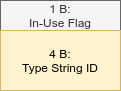
\includegraphics[keepaspectratio,height=0.2\textheight,width=0.2\textwidth]{img/relationship/rel_type_record.png}
        \end{center}
        \caption{A visualization of the record structure of a relationship type.} %TODO citation
    \end{figure}
    
    \subsubsection{Relationship Groups}~\label{rel_group}
    The relationship group record is used for example for dense nodes in order not to iterate over all relationships but only over those of a specific type. Each record consists of 25 bytes where the first byte again contains the in-use flags and the high order bits of IDs that do not fit into integers. The next bytes again contains high bits of addresses and is followed by the relationship type. After that a reference (an ID) to the next relationship group record is given. Finally the first outgoing relation, the first incoming relation, the first looping relation and the node of interest are specified.
    
    \begin{figure}[H]\label{rel_group_record}
        \begin{center}
            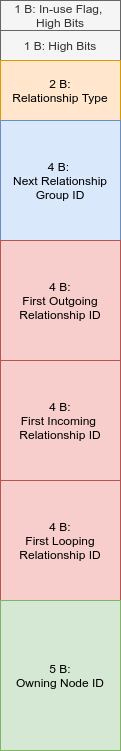
\includegraphics[keepaspectratio,height=0.2\textheight,width=0.2\textwidth]{img/relationship/relationship_group_record.png}
        \end{center}
        \caption{A visualization of the record structure of a relationship group.} %TODO citation
    \end{figure}
    
    \begin{enumerate}
     \item Byte 1: In-use flag, high bits for the next relationship group ID, high bits for the first entry of outgoing relationship list.
     \item Byte 2: High bits for the first entry in the incoming relationship list, high bits for the first entry in the looping relationship list.
     \item Bytes 3 and 4: Relationship type ID
     \item Bytes 5 - 8: ID of the next relationship group record.
     \item Bytes 9 - 12: ID of the first relationship in the linked list of outgoing relationships, i.e. those relationships which start at the record owning node.
     \item Bytes 13 - 16: ID of the first relationship in the linked list of incoming relationships, i.e. those relationships which end at the record owning node.
     \item Bytes 17 - 20: ID of the first relationship in the linked list of loops, i.e. relationships which start and end at the record owning node.
     \item Bytes 21 - 25: ID of the node for which the relationship group was created, also called the owning node (in the source code).
    \end{enumerate}
    
    \begin{figure}[H]\label{rel_group_first_bytes}
        \begin{center}
            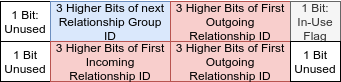
\includegraphics[keepaspectratio,height=0.2\textheight,width=0.2\textwidth]{img/relationship/relationship_group_first_bytes.png}
        \end{center}
        \caption{The structure of the first two bytes of a relationship group record.} %TODO citation
    \end{figure}
    

    \subsubsection{Properties}
    \begin{enumerate}
     \item 
    \end{enumerate}
    
    \subsubsection{Dynamic Records: Strings \& Arrays}\label{dynamic}
            
    \subsubsection{Other Records}
        TODO later
        \subsubsection{Schema}
        \subsubsection{Metadata}
        
        
    \subsubsection{Record Allocation}
        \href{https://neo4j.com/docs/operations-manual/current/performance/space-reuse/\#space-reuse}{Reusing space} \\
\href{https://neo4j.com/developer/kb/how-deletes-workin-neo4j/}{How delete works} \\
    
    \subsection{Record Allocation}

    \subsection{Indexes}
        TODO later
    

    
    
    


\href{https://neo4j.com/developer/kb/understanding-data-on-disk/}{Layout N4J} \\
\href{https://www.slideshare.net/thobe/an-overview-of-neo4j-internals}{Slides: Internals Of N4J} \\
\href{https://skillsmatter.com/skillscasts/2968-neo4j-internals}{Video} \\
\href{http://key-value-stories.blogspot.com/2015/02/neo4j-architecture.html}{N4J Arch blog} \\
\href{https://groups.google.com/g/neo4j/c/cxClivwF94k}{Followup discussion w devs}


\section{Examples}
\subsection{Relationship-focused Disk Access}
    \subsubsection{BFS Traversal}

    \subsubsection{Dijkstra Traversal}

    \subsubsection{A*-Traversal}

\subsection{All-files Disk Access}
 \subsubsection{BFS Traversal}

    \subsubsection{Dijkstra Traversal}

    \subsubsection{A*-Traversal}

\subsection{Caching-assisted Disk Access}
 \subsubsection{BFS Traversal}

    \subsubsection{Dijkstra Traversal}

    \subsubsection{A*-Traversal}


\section{Conclusion}


\end{document}
